% This is the Reed College LaTeX thesis template. Most of the work
% for the document class was done by Sam Noble (SN), as well as this
% template. Later comments etc. by Ben Salzberg (BTS). Additional
% restructuring and APA support by Jess Youngberg (JY).
% Your comments and suggestions are more than welcome; please email
% them to cus@reed.edu
%
% See http://web.reed.edu/cis/help/latex.html for help. There are a
% great bunch of help pages there, with notes on
% getting started, bibtex, etc. Go there and read it if you're not
% already familiar with LaTeX.
%
% Any line that starts with a percent symbol is a comment.
% They won't show up in the document, and are useful for notes
% to yourself and explaining commands.
% Commenting also removes a line from the document;
% very handy for troubleshooting problems. -BTS

% As far as I know, this follows the requirements laid out in
% the 2002-2003 Senior Handbook. Ask a librarian to check the
% document before binding. -SN

%%
%% Preamble
%%
% \documentclass{<something>} must begin each LaTeX document
\documentclass[12pt,twoside]{reedthesis}
% Packages are extensions to the basic LaTeX functions. Whatever you
% want to typeset, there is probably a package out there for it.
% Chemistry (chemtex), screenplays, you name it.
% Check out CTAN to see: http://www.ctan.org/
%%
\usepackage{graphicx,latexsym}
\usepackage{amssymb,amsthm,amsmath}
\usepackage{longtable,booktabs,setspace}
\usepackage{chemarr} %% Useful for one reaction arrow, useless if you're not a chem major
\usepackage[hyphens]{url}
\usepackage{rotating}
\usepackage{natbib}
% Comment out the natbib line above and uncomment the following two lines to use the new
% biblatex-chicago style, for Chicago A. Also make some changes at the end where the
% bibliography is included.
%\usepackage{biblatex-chicago}
%\bibliography{thesis}

% \usepackage{times} % other fonts are available like times, bookman, charter, palatino

\title{My Final College Paper}
\author{Sebastian Andrada Ottonello}
% The month and year that you submit your FINAL draft TO THE LIBRARY (May or December)
\date{May 2024}
\division{Mathematical and Natural Sciences}
\advisor{Charles McGuffey}
%If you have two advisors for some reason, you can use the following
%\altadvisor{Your Other Advisor}
%%% Remember to use the correct department!
\department{Computer Science}
% if you're writing a thesis in an interdisciplinary major,
% uncomment the line below and change the text as appropriate.
% check the Senior Handbook if unsure.
%\thedivisionof{The Established Interdisciplinary Committee for}
% if you want the approval page to say "Approved for the Committee",
% uncomment the next line
%\approvedforthe{Committee}

\setlength{\parskip}{0pt}
%%
%% End Preamble
%%
%% The fun begins:
\begin{document}

\maketitle
\frontmatter % this stuff will be roman-numbered
\pagestyle{empty} % this removes page numbers from the frontmatter

% Acknowledgements (Acceptable American spelling) are optional
% So are Acknowledgments (proper English spelling)
\chapter*{Acknowledgements}
I want to thank a few people.

% The preface is optional
% To remove it, comment it out or delete it.
\chapter*{Preface}
This is an example of a thesis setup to use the reed thesis document class.



\chapter*{List of Abbreviations}
You can always change the way your abbreviations are formatted. Play around with it yourself, use tables, or come to CUS if you'd like to change the way it looks. You can also completely remove this chapter if you have no need for a list of abbreviations. Here is an example of what this could look like:

\begin{table}[h]
	\centering % You could remove this to move table to the left
	\begin{tabular}{ll}
		\textbf{ALU}    & Arithmetic Logic Unit                 \\
		\textbf{CISC}   & Complex Instruction Set Computer      \\
		\textbf{CPU}    & Central Processing Unit               \\
		\textbf{ISA}    & Instruction Set Architecture          \\
		\textbf{RISC}   & Reduced Instruction Set Computer      \\
		\textbf{RISC-V} & Reduced Instruction Set Computer Five \\
	\end{tabular}
\end{table}


\tableofcontents
% if you want a list of tables, optional
\listoftables
% if you want a list of figures, also optional
\listoffigures

% The abstract is not required if you're writing a creative thesis (but aren't they all?)
% If your abstract is longer than a page, there may be a formatting issue.
\chapter*{Abstract}
The preface pretty much says it all.

\chapter*{Dedication}
You can have a dedication here if you wish.

\mainmatter % here the regular arabic numbering starts
\pagestyle{fancyplain} % turns page numbering back on

%The \introduction command is provided as a convenience.
%if you want special chapter formatting, you'll probably want to avoid using it altogether

\chapter*{Introduction}
\addcontentsline{toc}{chapter}{Introduction}
\chaptermark{Introduction}
\markboth{Introduction}{Introduction}
% The three lines above are to make sure that the headers are right, that the intro gets included in the table of contents, and that it doesn't get numbered 1 so that chapter one is 1.

% Double spacing: if you want to double space, or one and a half
% space, uncomment one of the following lines. You can go back to
% single spacing with the \singlespacing command.
% \onehalfspacing
% \doublespacing

Though there's countless pieces of hardware to study and delve into within this field, the CPU (Central Processing Unit) can be argued to be the most essential one. It is the heart of any computer, the piece that actually carries out the programs and computations that it was built for. It comes as no surprise, then, that most college-level Computer Systems courses begin by taking a close look at the inner workings of a simple CPU, so that they can then begin to understand how the other components of a computer support its functionality, and how it can produce computation out of just an assembly program, wires, and logic gates. Learning of this is all well and good, but getting hands-on experience with the topic is harder than one might expect: The powerful CPUs in the personal computers of students run on are all closed-source designs that obfuscate how they carry out their instructions; and even if they were transparent, the sheer breadth and depth of modifications they employ to get the performance they do would make their design completely indecipherable to a novice.

Therefore, the aim of this project is to develop a pedagogical simulator program, developed in the Rust programming language and capable of running on modern computers, that simulates a simple RISC-V CPU at the hardware level, running assembly code and then transparently displaying how the code and computed information traverse the inside of the processor. While simple, the simulated CPU implements a 5-stage pipeline design similar to the ones that are mandatory for modern CPUs. The project also seeks to include some user-facing features, like a graphical interface and the ability to step through and rewind through the execution of a program, to make the simulator more intuitive to use.

\chapter*{Background}
\section{What is an ISAs?}

But first, what does it even mean that the CPU is RISC-V? RISC-V is one of many ISAs, belonging to the RISC family of design.

Starting from the top, ISA stands for Instruction Set Architecture; you may have also heard it reffered to as just a CPU's "architecture", or of popular ISAs like x86 and ARM. We will go into the details later, but for now an ISA is simply a list of machine-code instructions that a CPU can carry out: These instructions are things like basic arithmetic operations (addition, subtraction, etc), calls to load or store data from the memory, or even jump instructions to alter the flow of the program. Ultimately, a program is just a list of these instructions, one after the other, that the CPU executes in order. A CPU is considered to use a certain ISA if it supports and has implemented all of its instructions. ISAs were created for the goal of hardware compatibility: As long as two different CPUs made by competing manufacturers both use the same ISA, any low-level program will run on both processors because they both guarantee that they'll support the same instruction set, no matter how different their underlying design is.

Ultimately, an ISA is a standard for how a CPU should take any given line of code from a low-level program - encoded as an integer in binary, this close to the hardware - and translate that into an actionable operation that the CPU should execute when it reaches that part of the program.

\section{Why RISC-V?}
Though the ISA doesn't ascribe an exact design for how its demands should be met(that's called the \textit{implementation}, and is the domain of the CPU's manufacturer), it so heavily shapes the CPU's capabilities, and therefore indirectly its design, that choosing which ISA to implement is the most important decision one can make when designing a CPU, whether it's real or virtual. As alluded to in the introduction, there are multiple ISAs to choose from, and many more popular ones than RISC-V. So, what makes competing ISAs so different from one another, and why choose RISC-V for this project instead of any of the more popular options?


RISC-V is a modern ISA, albeit one that has not yet experienced widespread success; while it very rapidly growing in use, its two contemporaries, x86 and ARM, dominate the Personal Computer CPU and Mobile CPU market entirely for the time being. And yet, RISC-V has two major advantages over them that make it the ideal choice for this simulator.

The first is, simply, that RISC-V is fully open source. Unlike its two proprietary cousins, the full listings of all the RISC-V instructions are freely available, with details on what behavior is expected of each instruction and exactly how to glean an instruction's parameter from its 32-bit integer representation. Working with open-source sorftware and specifications is good by its very nature in that its development benefits everyone, not just its creators, but it's also a better choice practically.

The second difference is that RISC-V is a RISC ISA, while x86 is a CISC ISA; it's even in the name. These stands for \textit{Reduced Instruction Set Computer} and \textit{Complex Instruction Set Computer} respectively, and they are opposing schools of design for an ISA. The difference ultimately comes down to how many different instructions the ISA lists out: The idea of a CISC ISA is that by providing a very large variety of different instructions, most individual things you'd want a program to do can be performed with just one instruction each. By contrast, a RISC ISA aims to keep its total number of instructions low: While this would mean that code would need more total instructions to accomplish the same task, the idea is that keeping the demands simpler would allow RISC processors to have faster and more efficient designs that offset this cost \footnote{\cite{denning}}. This also coincidentally makes RISC processors a much better example for students to study, while still remaining a modern architecture that's growing in widespread use.

\section{An abstract view of how a CPU functions}
In order to build and understand the design of a CPU, we must first understand what it, in general terms, does. We've already established that a CPU carries out a program consisting of instructions from its ISA. However, what exactly do those instructions demand the CPU do, and what does the CPU have access to to carry it out?

We will go over the exact design of the model of CPU shown here later, with all of its intricacies and small parts. But, in broad terms, the CPU has access to: an \textbf{Instruction Memory}, where the program to be executed is stored instruction-by-instruction. A \textbf{Decoder} that reads this raw 32-bit instruction and gleans the important details from it, like what instruction it is, what the inputs and outputs are, or other instruction-specific data. A \textbf{Register Memory}, which holds a small amount of numbered registers that store information; think of them as set mini-variables built directly into the CPU that it has quick and easy access to. A \textbf{Data Memory}, external and much larger than the previous two, in which to store larger values; and finally an \textbf{ALU}, Arithmetic Logic Unit, which is simply capable of performing arithmetic operations on the values it is given. This explanation leaves out many crucial components and smaller parts that make the whole thing possible, but they're enough to understand the CPU's general plan, detailed here below. Note that this plan, and the designs described later, do not accurately describe all CPUs; rather, it is a simple design that, despite that, is fully equipped to execute base RISC-V programs. (REDO AS FOOTNOTE?)

1. Read the first instruction from the Instruction Memory.\textbf{(IF: Instruction Fetch)}

2. Decode the fetched instruction, and read the values of whichever registers the instruction calls for. \textbf{(ID: Instruction Decode)}

3. Perform whichever arithmetic operation the instruction calls for, using values from the registers or from the instruction itself as input. \textbf{(EX: Execute)}

4. If the instruction calls for a value to be read from or stored to the Data Memory, do so. \textbf{(MEM: Memory)}

5. Write back the end-result value of the instruction into the destination register it specified. \textbf{(WB: WriteBack)}

6. Read the next instruction from the Instruction Memory, and start over again at step 2. Repeat until end of program.

These five repeating steps, called stages, are enough to accomplish everything that base version of RISC-V calls for, shockingly! It is enough for the CPU to successfully run low-level programs. How these simple instructions build up to the complex operating systems and graphical applications that most are familiar with today is beyond the scope of this project, but the important thing is that it is enough.

Do note that the dividing of the process of executing one instruction into five steps is arbitrary. However, this arbitrary 5-stage model is going to be incredibly helpful to implementing the pipeline design/feature of this simulator, which will be described later.

It is also enough to get a rough idea of how any given RISC-V instruction is carried out. The full list of instructions can be found on the official \textit{RISC-V Instruction Set Manual} that is freely available online, or on a number of more user-friendly guides like Five EmbedDev's \textit{RISC-V ISA Instruction Quick Reference}. A list of all the instructions in the most basic version of RISC-V, the RV32I Base Integer Instruction Set, can be found (INSERT HERE), but the instructions are broadly divided into the following four categories by the \textit{RISC-V Instruction Set Manual}:


\textbf{Register-Register Computation:} These instructions take two registers as input, perform some sort of operation on their two values (an arithmetic operation like addition, or a logical operation like a bitwise AND or NOT), and store the result in a third register.

\textbf{Register-Immediate Computation:} These are the same as RR (Register-Register) instructions, but take as input one register and one hard-coded value that's written directly into the program, called an Immediate. It's the difference between "z = x + y" and "z = x + 3".

\textbf{Load/Store:} The purpose of these instructions are simply to interact with the Data Memory, either storing a value to a specific address or reading a value from it.

\textbf{Control Transfer:} Instructions that call for the CPU to move on to a place in the code that is NOT the next instruction, potentially. These are what make the If-Then statements and Loops of high-level programming languages possible. These work because there is a simple \textbf{Program Counter}, PC, attached to the Instruction Memory that simply keeps track of which instruction should be performed next.

Each of these instructions in these categories, conveniently, move through the 5-stage process in roughly the same way based on their category.

\textbf{RR Computation:} Run through the steps as usual, feeding the value of its two input registers as the input for the ALU. ignore step 4, MEM, since Comptutational Instructions do not interact with the Data Memory.

\textbf{RI Computation:} Same as RR; but only one register is read at step 2. the other input value is the immediate, which the Decoder reads from the instruction itself.

\textbf{Load:} Load Instructions have a Register and an Immediate as input, representing the address in data memory to read from, as well as a destination register. They run through all of the steps; in the EX stage, the register value and immediate are added together to get the final address, which is then fed to the Data Memory in the MEM stage. Finally, the data loaded from Data Memory is stored in the destination register.

\textbf{Store:} Store Instructions are similar to Load, but have two registers and an Immediate, with no destination register. The first register + Immediate are the address as usual, but the second register holds the value that is to be stored into memory; and is sent directly to the Data Memory through its own special wire.

\textbf{Control Transfer:} Control Transfer Instructions have an Immediate that describes where the program should jump to, and possibly some registers. They run normally until the EX stage: Here, rather than operate on registers, the ALU is given the Immediate and the current value of the PC, which are added together to determine the Jump location. Some additional computation may be performed in this stage, such as a comparison between registers, and for some instructions the jump destination is written to an output register, but the CPU, at this point, goes back to the IF stage while editing the value of the Program Counter to complete the jump.

\section{A more detailed look of how a CPU functions}

This information is enough to build a full hardware model of the CPU that the simulator will use; at least if Pipelining is ignored for now. The following is a visual representation of this model:

(INSERT DIAGRAM HERE)

Most of the components shown here have already been explained earlier, albeit with some modifications and additions. It should be noted that the components are arranged from left to right in the order of the stages; with the wires of the WB stage looping back to where the outputs should be stored. The notable changes are as follows:

1. The decoder is actually two components: The Decoder and the Immediates Decoder. The Decoder focuses on getting the indices of the two input registers and the destination register; and then a set of values called the opcode, funct3, and funct7. These are 8-bit, 3-bit, and 7-bit numbers respectively that, together, describe which exact instruction it is. The Immediates code gets the opcode in order to get the immediates out of the instruction; depending on the exact instruction, the immediate is found in different bits; RR instructions have no immediates at all.

2. There is a Branch Comparator component alongside the ALU. This allows Branch instructions to, while the ALU is busy computing the final destination of the jump, calculate whether the jump should happen or not.

3. Lastly, there are multiplexors, drawn as (INSERT INFO HERE), throughout. These simply take multiple inputs and, based on the state of the CPU, decide which one should pass through. For example, the two multiplexors right before the ALU need to decide to let the values from registers r1 and r2 pass on an RR instruction, but let the current PC and the Immediate pass in during a Control Transfer instruction.

This is enough to understand the CPU simulator, for the most part; rather than simply take in a machine-code program and execute it as efficiently as possible, which would be trivial to do in a modern high-level programming language, the simulator represents each of these components individually as structs, so that the flow of data through the CPU circuits can be displayed accurately. 

\section{CPU-Simulator Features}

\section{Pipelining}

However, there is one feature for which the previous CPU diagram is not accurate; it requires alterations to it to be implemented. However, this feature is quite powerful, and used near-universally in RISC-V CPU designs (CITATION NEEDED), and so the simulator is designed with it in mind.

The current design has one simple issue: It is painfully slow. This design is capable of executing one instruction per cycle: one instruction per full use of each of the CPU's parts. This may seem good, but at any given moment, most of the CPU is actually going unused: The decoder is waiting on the instruction memory to fetch the instruction it needs to decode, which is waited upon by the register memory that needs the register indices to fetch their data, which is waited upon by the ALU that wants its inputs, so on. When, say, the ALU is firing and computing, the data memory, decoder, instruction memory, ETC, are all entirely dormant. They could, theoretically, be doing something useful at the same time; but because our design handles one instruction at a time, the components before the ALU have already done their part and the components after the ALU are waiting on it to finish and present its output. Theoretically, one could be multiplying efficiency of this CPU many times.

(DIAGRAM HERE OF THE STEPS, SHOW WASTED SPACE )

The solution is simple in theory, though difficult in execution: have the CPU be performing multiple instructions at once. Five of them, to be exact. This is where the five stages come into play: each stage does its part, performing its needed function for the current instruction; but when that instruction is passed off to the next stage, rather than waiting around for the full round trip, it's already receiving the information for the next instruction right away. If the WB stage is executing instruction number 9, the MEM stage is executing instruction 8, and the EX is executing instruction 7, so on.

(FOOTNOTE??)

(DIAGRAM HERE OF THE PIPELINED STEPS)

This is much, much faster;  in optimal conditions, the CPU can execute 5 instructions per cycle! Of course, conditions are not always optimal. A certain addition will be needed to this diagram for pipelining to be possible at all; A few smaller ones will be needed to handle new issues that arise out of pipelining specifically; and some of those new issues can only be mitigated, not avoided fully. Let's go over these.

The first modification, which makes pipelining possible on a basic level, is to handle coordination. Theoretically, if  every subcomponent of a CPU was perfectly coordinated and each of the five stages each always took the exact same amount of time to complete, one could simply set the CPU going, with a slight alteration to the PC so that it increments its program count 5 times per cycle instead of once. However, this is not the case: In real hardware, one cannot count on parts being perfectly coordinated; and some stages will take more or less time than others. The memory stage, notably, can require time to perform that is magnitudes longer than the other stages when it is required to go off the CPU and into a separate RAM stick, as is often used in more complex modern computers. (NEED FIXING/CITATION) Data memory structures even tend to have specialized on-CPU caches to minimize the need for this; it was originally intended for the CPU simulator to represent these fully as well, but this was proven to be beyond the scope of the project. Instead, the Data Memory is abstracted as a "black-box" subcomponent, which stores an array of data accessible by address through unknown means. Indeed, this entire timing aspect will be largely abstracted away in the simulator, operating entirely on the time unit of a "step" in which each of the instructions currently in the CPU advance by one stage; however, the alteration used to solve this timing issue in real hardware is so essential to the design, and additionally used in some of the solutions for smaller problems that cannot be abstracted away, that they will be included in the simulator regardless. 

So, what is this modification? The main thing to be prevented here is that no stage of the CPU should recieve the inputs for the next instruction before it is done performing its computations for its current structure; to keep all five stages in sync. The ideal way to do this is to "hold" the outputs of each stage once they are computed, until the slowest stage completes its computations, and then release them all at once to begin the next step. This "holding" of outputs is done through the addition of a set of "Latches" to the CPU: 

(INSERT CPU + LATCHES DIAGRAM)

There's one latch inbetween each CPU stage, with all of the outputs passing through said latch. They are named after the two stages they separate, with the leftmost being the "IF-ID Latch" for example. No latch is needed after WB, since that stage simply consists of delivering the instruction result to where it needs to go. The latches have two states: "Open" and "Closed". When the latch is "open", all the circuits operate as normal, as if the latch wasn't even there. When it is closed, the latch "blocks" the incoming inputs while keeping the outputs unchanging: If the ALU's output wire read "13" before the EX-MEM latch was closed, and "4" after, the latch will continue to output "13" to the wire leading from the latch to the Data Memory until the latch is opened again. This achieves the 'holding' effect that was desired, and makes pipelining possible at all! In order to pipeline possible... (REFRESH ON HARDWARE LEVEL OF LATCH OPERATION)

However, even with pipeline and latches in place, there are still other issues that will arise. Ultimately, whoever wrote the code that this CPU is running did so under the fundamental assumption that the CPU executes one instruction of code after the other, sequentially, waiting to finish one instruction before beginning the next. This is not the case in our faster, pipelined CPU; and while that's fine in most cases, it isn't always. There are certain scenarios that can occur in a machine code program where, due to this false assumption, our pipelined CPU as-it-is will produce an output that is wildly different from what the program correctly should. These scenarios are called "Hazards" In order for the pipelined CPU model to be valid, it must  have some way to avoid or correct any hazards that come up! Hazards can be broadly divided into these groups:

- Data Hazards: Hazards that involve the reading and writing of data to registers.

- Branch Hazards: Hazards that involve conditional/branching jump instructions.

(... WERE THERE MORE??)

Let's look at these hazards in more details, and at how the pipeline CPU design can be altereted to handle them.

\section{Data Hazards}



\section{Bibliographies}
Of course you will need to cite things, and you will probably accumulate an armful of sources. This is why BibTeX was created. For more information about BibTeX and bibliographies, see our CUS site (\url{web.reed.edu/cis/help/latex/index.html})\footnote{\cite{reedweb:2007}}. There are three pages on this topic: {\it bibtex} (which talks about using BibTeX, at \url{/latex/bibtex.html}), {\it bibtexstyles} (about how to find and use the bibliography style that best suits your needs, at \url{/latex/bibtexstyles.html}) and {\it bibman} (which covers how to make and maintain a bibliography by hand, without BibTeX, at at \url{/latex/bibman.html}). The last page will not be useful unless you have only a few sources. There used to be APA stuff here, but we don't need it since I've fixed this with my apa-good natbib style file.

\subsection{Tips for Bibliographies}
\begin{enumerate}
	\item Like with thesis formatting, the sooner you start compiling your bibliography for something as large as thesis, the better. Typing in source after source is mind-numbing enough; do you really want to do it for hours on end in late April? Think of it as procrastination.
	\item The cite key (a citation's label) needs to be unique from the other entries.
	\item When you have more than one author or editor, you need to separate each author's name by the word ``and'' e.g.\\ \verb+Author = {Noble, Sam and Youngberg, Jessica},+.
	\item Bibliographies made using BibTeX (whether manually or using a manager) accept LaTeX markup, so you can italicize and add symbols as necessary.
	\item To force capitalization in an article title or where all lowercase is generally used, bracket the capital letter in curly braces.
	\item You can add a Reed Thesis citation\footnote{\cite{noble:2002}} option. The best way to do this is to use the phdthesis type of citation, and use the optional ``type'' field to enter ``Reed thesis'' or ``Undergraduate thesis''. Here's a test of Chicago, showing the second cite in a row\footnote{\cite{noble:2002}} being different. Also the second time not in a row\footnote{\cite{reedweb:2007}} should be different. Of course in other styles they'll all look the same.
\end{enumerate}
\section{Anything else?}
If you'd like to see examples of other things in this template, please contact CUS (email cus@reed.edu) with your suggestions. We love to see people using \LaTeX\ for their theses, and are happy to help.


\chapter{Mathematics and Science}
\section{Math}
\TeX\ is the best way to typeset mathematics. Donald Knuth designed \TeX\ when he got frustrated at how long it was taking the typesetters to finish his book, which contained a lot of mathematics.

If you are doing a thesis that will involve lots of math, you will want to read the following section which has been commented out. If you're not going to use math, skip over this next big red section. (It's red in the .tex file but does not show up in the .pdf.)
%
%% MATH and PHYSICS majors: Uncomment the following section
%	$$\sum_{j=1}^n (\delta\theta_j)^2 \leq {{\beta_i^2}\over{\delta_i^2 + \rho_i^2}}
%\left[ 2\rho_i^2 + {\delta_i^2\beta_i^2\over{\delta_i^2 + \rho_i^2}} \right] \equiv \omega_i^2
%$$

%From Informational Dynamics, we have the following (Dave Braden):

%After {\it n} such encounters the posterior density for $\theta$ is

%$$
%\pi(\theta|X_1< y_1,\dots,X_n<y_n) \varpropto \pi(\theta) \prod_{i=1}^n\int_{-\infty}^{y_i}
%   \exp\left(-{(x-\theta)^2\over{2\sigma^2}}\right)\ dx
%$$

%

%Another equation:

%$$\det\left|\,\begin{matrix}%
%c_0&c_1\hfill&c_2\hfill&\ldots&c_n\hfill\cr
%c_1&c_2\hfill&c_3\hfill&\ldots&c_{n+1}\hfill\cr
%c_2&c_3\hfill&c_4\hfill&\ldots&c_{n+2}\hfill\cr
%\,\vdots\hfill&\,\vdots\hfill&
%  \,\vdots\hfill&&\,\vdots\hfill\cr
%c_n&c_{n+1}\hfill&c_{n+2}\hfill&\ldots&c_{2n}\hfill\cr
%\end{matrix}\right|>0$$

%
%Lapidus and Pindar, Numerical Solution of Partial Differential Equations in Science and
%Engineering.  Page 54

%$$
%\int_t\left\{\sum_{j=1}^3 T_j \left({d\phi_j\over dt}+k\phi_j\right)-kT_e\right\}w_i(t)\ dt=0,
%   \qquad\quad i=1,2,3.
%$$

%L\&P  Galerkin method weighting functions.  Page 55

%$$
%\sum_{j=1}^3 T_j\int_0^1\left\{{d\phi_j\over dt} + k\phi_j\right\} \phi_i\ dt
%   = \int_{0}^1k\,T_e\phi_idt, \qquad i=1,2,3 $$
%
%Another L\&P (p145)

%$$
%\int_{-1}^1\!\int_{-1}^1\!\int_{-1}^1 f\big(\xi,\eta,\zeta\big)
%   = \sum_{k=1}^n\sum_{j=1}^n\sum_{i=1}^n w_i w_j w_k f\big( \xi,\eta,\zeta\big).
%$$

%Another L\&P (p126)

%$$
%\int_{A_e} (\,\cdot\,) dx dy = \int_{-1}^1\!\int_{-1}^1 (\,\cdot\,) \det[J] d\xi d\eta.
%$$

\section{Chemistry 101: Symbols}
Chemical formulas will look best if they are not italicized. Get around math mode's automatic italicizing by using the argument \verb=$\mathrm{formula here}$=, with your formula inside the curly brackets.

So, $\mathrm{Fe_2^{2+}Cr_2O_4}$ is written \verb=$\mathrm{Fe_2^{2+}Cr_2O_4}$=\\
Exponent or Superscript: O$^{-}$\\
Subscript: CH$_{4}$\\

To stack numbers or letters as in $\mathrm{Fe_2^{2+}}$, the subscript is defined first, and then the superscript is defined.\\
Angstrom: {\AA}\\
Bullet: CuCl $\bullet$ 7H${_2}$O\\
Double Dagger: \ddag \/\\
Delta: $\Delta$\\
Reaction Arrows: $\longrightarrow$ or  $\xrightarrow{solution}$\\
Resonance Arrows: $\leftrightarrow$\\
Reversible Reaction Arrows: $\rightleftharpoons$ or $\xrightleftharpoons[ ]{solution}$ (the latter requires the chemarr package)\\


\subsection{Typesetting reactions}
You may wish to put your reaction in a figure environment, which means that LaTeX will place the reaction where it fits and you can have a figure legend if desired:
\begin{figure}[htbp]
	\begin{center}
		$\mathrm{C_6H_{12}O_6  + 6O_2} \longrightarrow \mathrm{6CO_2 + 6H_2O}$
		\caption{Combustion of glucose}
		\label{combustion of glucose}
	\end{center}
\end{figure}

\subsection{Other examples of reactions}
$\mathrm{NH_4Cl_{(s)}} \rightleftharpoons \mathrm{NH_{3(g)}+HCl_{(g)}}$\\
$\mathrm{MeCH_2Br + Mg} \xrightarrow[below]{above} \mathrm{MeCH_2\bullet Mg \bullet Br}$

\section{Physics}

Many of the symbols you will need can be found on the math page (\url{http://web.reed.edu/cis/help/latex/math.html}) and the Comprehensive \LaTeX\ Symbol Guide (enclosed in this template download).  You may wish to create custom commands for commonly used symbols, phrases or equations, as described in Chapter \ref{commands}.

\section{Biology}
You will probably find the resources at \url{http://www.lecb.ncifcrf.gov/~toms/latex.html} helpful, particularly the links to bsts for various journals. You may also be interested in TeXShade for nucleotide typesetting (\url{http://homepages.uni-tuebingen.de/beitz/txe.html}).  Be sure to read the proceeding chapter on graphics and tables, and remember that the thesis template has versions of Ecology and Science bsts which support webpage citation formats.

\chapter{Tables and Graphics}

\section{Tables}
The following section contains examples of tables, most of which have been commented out for brevity. (They will show up in the .tex document in red, but not at all in the .pdf). For more help in constructing a table (or anything else in this document), please see the LaTeX pages on the CUS site.

\begin{table}[htbp] % begins the table floating environment. This enables LaTeX to fit the table where it works best and lets you add a caption.
	\caption[Correlation of Inheritance Factors between Parents and Child]{Correlation of Inheritance Factors between Parents and Child}
	% The words in square brackets of the caption command end up in the Table of Tables. The words in curly braces are the caption directly over the table.
	\begin{center}
		% makes the table centered
		\begin{tabular}{c c c c}
			% the tabular environment is used to make the table itself. The {c c c c} specify that the table will have four columns and they will all be center-aligned. You can make the cell contents left aligned by replacing the Cs with Ls or right aligned by using Rs instead. Add more letters for more columns, and pipes (the vertical line above the backslash) for vertical lines. Another useful type of column is the p{width} column, which forces text to wrap within whatever width you specify e.g. p{1in}. Text will wrap badly in narrow columns though, so beware.
			\toprule % a horizontal line, slightly thicker than \hline, depends on the booktabs package
			Factors               & Correlation between Parents \& Child & Inherited \\ % the first row of the table. Separate columns with ampersands and end the line with two backslashes. An environment begun in one cell will not carry over to adjacent rows.
			\midrule % another horizontal line
			Education             & -0.49                                & Yes       \\ % another row
			Socio-Economic Status & 0.28                                 & Slight    \\
			Income                & 0.08                                 & No        \\
			Family Size           & 0.19                                 & Slight    \\
			Occupational Prestige & 0.21                                 & Slight    \\
			\bottomrule % yet another horizontal line
		\end{tabular}
	\end{center}
	\label{inheritance} % labels are useful when you have more than one table or figure in your document. See our online documentation for more on this.
\end{table}

\clearpage
%% \clearpage ends the page, and also dumps out all floats.
%% Floats are things like tables and figures.

If you want to make a table that is longer than a page, you will want to use the longtable environment. Uncomment the table below to see an example, or see our online documentation.

%% An example of a long table, with headers that repeat on each subsequent page: Results from the summers of 1998 and 1999 work at Reed College done by Grace Brannigan, Robert Holiday and Lien Ngo in 1998 and Kate Brown and Christina Inman in 1999.

\begin{longtable}{||c|c|c|c||}
	\caption[Chromium Hexacarbonyl Data Collected in 1998--1999]{Chromium Hexacarbonyl Data Collected in 1998--1999} \\ \hline
	\multicolumn{4}{||c||}{Chromium Hexacarbonyl}                                                                    \\\hline
	State                & Laser wavelength & Buffer gas & Ratio of $\frac{\textrm{Intensity
	at vapor pressure}}{\textrm{Intensity at 240 Torr}}$                                                             \\ \hline
	\endfirsthead
	\hline     State     & Laser wavelength & Buffer gas & Ratio of
	$\frac{\textrm{Intensity at vapor pressure}}{\textrm{Intensity at 240 Torr}}$                                    \\
	\hline
	\endhead

	$z^{7}P^{\circ}_{4}$ & 266 nm           & Argon      & 1.5                                                       \\\hline
	$z^{7}P^{\circ}_{2}$ & 355 nm           & Argon      & 0.57                                                      \\\hline
	$y^{7}P^{\circ}_{3}$ & 266 nm           & Argon      & 1                                                         \\\hline
	$y^{7}P^{\circ}_{3}$ & 355 nm           & Argon      & 0.14                                                      \\\hline
	$y^{7}P^{\circ}_{2}$ & 355 nm           & Argon      & 0.14                                                      \\\hline
	$z^{5}P^{\circ}_{3}$ & 266 nm           & Argon      & 1.2                                                       \\\hline
	$z^{5}P^{\circ}_{3}$ & 355 nm           & Argon      & 0.04                                                      \\\hline
	$z^{5}P^{\circ}_{3}$ & 355 nm           & Helium     & 0.02                                                      \\\hline
	$z^{5}P^{\circ}_{2}$ & 355 nm           & Argon      & 0.07                                                      \\\hline
	$z^{5}P^{\circ}_{1}$ & 355 nm           & Argon      & 0.05                                                      \\\hline
	$y^{5}P^{\circ}_{3}$ & 355 nm           & Argon      & 0.05, 0.4                                                 \\\hline
	$y^{5}P^{\circ}_{3}$ & 355 nm           & Helium     & 0.25                                                      \\\hline
	$z^{5}F^{\circ}_{4}$ & 266 nm           & Argon      & 1.4                                                       \\\hline
	$z^{5}F^{\circ}_{4}$ & 355 nm           & Argon      & 0.29                                                      \\\hline
	$z^{5}F^{\circ}_{4}$ & 355 nm           & Helium     & 1.02                                                      \\\hline
	$z^{5}D^{\circ}_{4}$ & 355 nm           & Argon      & 0.3                                                       \\\hline
	$z^{5}D^{\circ}_{4}$ & 355 nm           & Helium     & 0.65                                                      \\\hline
	$y^{5}H^{\circ}_{7}$ & 266 nm           & Argon      & 0.17                                                      \\\hline
	$y^{5}H^{\circ}_{7}$ & 355 nm           & Argon      & 0.13                                                      \\\hline
	$y^{5}H^{\circ}_{7}$ & 355 nm           & Helium     & 0.11                                                      \\\hline
	$a^{5}D_{3}$         & 266 nm           & Argon      & 0.71                                                      \\\hline
	$a^{5}D_{2}$         & 266 nm           & Argon      & 0.77                                                      \\\hline
	$a^{5}D_{2}$         & 355 nm           & Argon      & 0.63                                                      \\\hline
	$a^{3}D_{3}$         & 355 nm           & Argon      & 0.05                                                      \\\hline
	$a^{5}S_{2}$         & 266 nm           & Argon      & 2                                                         \\\hline
	$a^{5}S_{2}$         & 355 nm           & Argon      & 1.5                                                       \\\hline
	$a^{5}G_{6}$         & 355 nm           & Argon      & 0.91                                                      \\\hline
	$a^{3}G_{4}$         & 355 nm           & Argon      & 0.08                                                      \\\hline
	$e^{7}D_{5}$         & 355 nm           & Helium     & 3.5                                                       \\\hline
	$e^{7}D_{3}$         & 355 nm           & Helium     & 3                                                         \\\hline
	$f^{7}D_{5}$         & 355 nm           & Helium     & 0.25                                                      \\\hline
	$f^{7}D_{5}$         & 355 nm           & Argon      & 0.25                                                      \\\hline
	$f^{7}D_{4}$         & 355 nm           & Argon      & 0.2                                                       \\\hline
	$f^{7}D_{4}$         & 355 nm           & Helium     & 0.3                                                       \\\hline
	\multicolumn{4}{||c||}{Propyl-ACT}                                                                               \\\hline
	%	    State & Laser wavelength & Buffer gas & Ratio of $\frac{\textrm{Intensity
	%at vapor pressure}}{\textrm{Intensity at 240 Torr}}$\\ \hline
	$z^{7}P^{\circ}_{4}$ & 355 nm           & Argon      & 1.5                                                       \\\hline
	$z^{7}P^{\circ}_{3}$ & 355 nm           & Argon      & 1.5                                                       \\\hline
	$z^{7}P^{\circ}_{2}$ & 355 nm           & Argon      & 1.25                                                      \\\hline
	$z^{7}F^{\circ}_{5}$ & 355 nm           & Argon      & 2.85                                                      \\\hline
	$y^{7}P^{\circ}_{4}$ & 355 nm           & Argon      & 0.07                                                      \\\hline
	$y^{7}P^{\circ}_{3}$ & 355 nm           & Argon      & 0.06                                                      \\\hline
	$z^{5}P^{\circ}_{3}$ & 355 nm           & Argon      & 0.12                                                      \\\hline
	$z^{5}P^{\circ}_{2}$ & 355 nm           & Argon      & 0.13                                                      \\\hline
	$z^{5}P^{\circ}_{1}$ & 355 nm           & Argon      & 0.14                                                      \\\hline
	\multicolumn{4}{||c||}{Methyl-ACT}                                                                               \\\hline
	%	    State & Laser wavelength & Buffer gas & Ratio of $\frac{\textrm{Intensity
	% at vapor pressure}}{\textrm{Intensity at 240 Torr}}$\\ \hline
	$z^{7}P^{\circ}_{4}$ & 355 nm           & Argon      & 1.6, 2.5                                                  \\\hline
	$z^{7}P^{\circ}_{4}$ & 355 nm           & Helium     & 3                                                         \\\hline
	$z^{7}P^{\circ}_{4}$ & 266 nm           & Argon      & 1.33                                                      \\\hline
	$z^{7}P^{\circ}_{3}$ & 355 nm           & Argon      & 1.5                                                       \\\hline
	$z^{7}P^{\circ}_{2}$ & 355 nm           & Argon      & 1.25, 1.3                                                 \\\hline
	$z^{7}F^{\circ}_{5}$ & 355 nm           & Argon      & 3                                                         \\\hline
	$y^{7}P^{\circ}_{4}$ & 355 nm           & Argon      & 0.07, 0.08                                                \\\hline
	$y^{7}P^{\circ}_{4}$ & 355 nm           & Helium     & 0.2                                                       \\\hline
	$y^{7}P^{\circ}_{3}$ & 266 nm           & Argon      & 1.22                                                      \\\hline
	$y^{7}P^{\circ}_{3}$ & 355 nm           & Argon      & 0.08                                                      \\\hline
	$y^{7}P^{\circ}_{2}$ & 355 nm           & Argon      & 0.1                                                       \\\hline
	$z^{5}P^{\circ}_{3}$ & 266 nm           & Argon      & 0.67                                                      \\\hline
	$z^{5}P^{\circ}_{3}$ & 355 nm           & Argon      & 0.08, 0.17                                                \\\hline
	$z^{5}P^{\circ}_{3}$ & 355 nm           & Helium     & 0.12                                                      \\\hline
	$z^{5}P^{\circ}_{2}$ & 355 nm           & Argon      & 0.13                                                      \\\hline
	$z^{5}P^{\circ}_{1}$ & 355 nm           & Argon      & 0.09                                                      \\\hline
	$y^{5}H^{\circ}_{7}$ & 355 nm           & Argon      & 0.06, 0.05                                                \\\hline
	$a^{5}D_{3}$         & 266 nm           & Argon      & 2.5                                                       \\\hline
	$a^{5}D_{2}$         & 266 nm           & Argon      & 1.9                                                       \\\hline
	$a^{5}D_{2}$         & 355 nm           & Argon      & 1.17                                                      \\\hline
	$a^{5}S_{2}$         & 266 nm           & Argon      & 2.3                                                       \\\hline
	$a^{5}S_{2}$         & 355 nm           & Argon      & 1.11                                                      \\\hline
	$a^{5}G_{6}$         & 355 nm           & Argon      & 1.6                                                       \\\hline
	$e^{7}D_{5}$         & 355 nm           & Argon      & 1                                                         \\\hline
\end{longtable}


\section{Figures}

If your thesis has a lot of figures, \LaTeX\ might behave better for you than that other word processor.  One thing that may be annoying is the way it handles ``floats'' like tables and figures. \LaTeX\ will try to find the best place to put your object based on the text around it and until you're really, truly done writing you should just leave it where it lies.   There are some optional arguments to the figure and table environments to specify where you want it to appear; see the comments in the first figure.

If you need a graphic or tabular material to be part of the text, you can just put it inline. If you need it to appear in the list of figures or tables, it should be placed in the floating environment.

To get a figure from StatView, JMP, SPSS or other statistics program into a figure, you can print to pdf or save the image as a jpg or png. Precisely how you will do this depends on the program: you may need to copy-paste figures into Photoshop or other graphic program, then save in the appropriate format.

Below we have put a few examples of figures. For more help using graphics and the float environment, see our online documentation.

And this is how you add a figure with a graphic:
\begin{figure}[h]
	% the options are h = here, t = top, b = bottom, p = page of figures.
	% you can add an exclamation mark to make it try harder, and multiple
	% options if you have an order of preference, e.g.
	% \begin{figure}[h!tbp]

	\centering
	% DO NOT ADD A FILENAME EXTENSION TO THE GRAPHIC FILE
	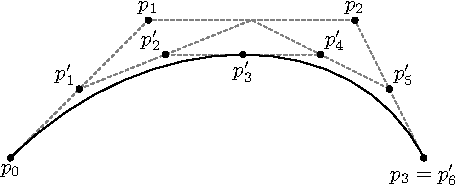
\includegraphics{subdivision}
	\caption{A Figure}
	\label{subd}
\end{figure}

\clearpage %% starts a new page and stops trying to place floats such as tables and figures

\section{More Figure Stuff}
You can also scale and rotate figures.
\begin{figure}[h!]

	\centering
	% DO NOT ADD A FILENAME EXTENSION TO THE GRAPHIC FILE
	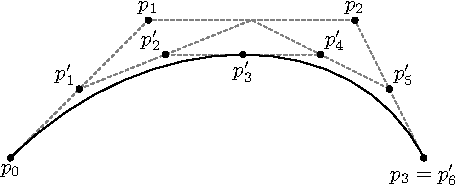
\includegraphics[scale=0.5,angle=180]{subdivision}
	% if your figure shows up not where you want it, it may just be too big to fit. You can use the scale argument to shrink it, e.g. scale=0.85 is 85 percent of the original size.
	\caption{A Smaller Figure, Flipped Upside Down}
	\label{subd2}
\end{figure}

\section{Even More Figure Stuff}
With some clever work you can crop a figure, which is handy if (for instance) your EPS or PDF is a little graphic on a whole sheet of paper. The viewport arguments are the lower-left and upper-right coordinates for the area you want to crop.

\begin{figure}[h!]
	\centering
	% DO NOT ADD A FILENAME EXTENSION TO THE GRAPHIC FILE
	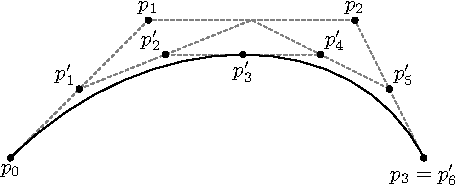
\includegraphics[clip=true, viewport=.0in .0in 1in 1in]{subdivision}
	\caption{A Cropped Figure}
	\label{subd3}
\end{figure}

\subsection{Common Modifications}
The following figure features the more popular changes thesis students want to their figures. This information is also on the web at \url{web.reed.edu/cis/help/latex/graphics.html}.
%\renewcommand{\thefigure}{0.\arabic{figure}} 	% Renumbers the figure to the type 0.x
%\addtocounter{figure}{4} 						% starts the figure numbering at 4
\begin{figure}[htbp]
	\begin{center}
		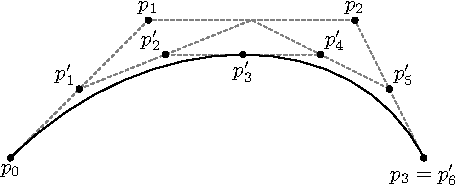
\includegraphics[scale=0.5]{subdivision}
		\caption[Subdivision of arc segments]{\footnotesize{Subdivision of arc segments. You can see that $ p_3 = p_6^\prime$.}} %the special ToC caption is in square brackets. The \footnotesize makes the figure caption smaller
		\label{barplot}
	\end{center}
\end{figure}

\chapter*{Conclusion}
\addcontentsline{toc}{chapter}{Conclusion}
\chaptermark{Conclusion}
\markboth{Conclusion}{Conclusion}
\setcounter{chapter}{4}
\setcounter{section}{0}

Here's a conclusion, demonstrating the use of all that manual incrementing and table of contents adding that has to happen if you use the starred form of the chapter command. The deal is, the chapter command in \LaTeX\ does a lot of things: it increments the chapter counter, it resets the section counter to zero, it puts the name of the chapter into the table of contents and the running headers, and probably some other stuff.

So, if you remove all that stuff because you don't like it to say ``Chapter 4: Conclusion'', then you have to manually add all the things \LaTeX\ would normally do for you. Maybe someday we'll write a new chapter macro that doesn't add ``Chapter X'' to the beginning of every chapter title.

\section{More info}
And here's some other random info: the first paragraph after a chapter title or section head \emph{shouldn't be} indented, because indents are to tell the reader that you're starting a new paragraph. Since that's obvious after a chapter or section title, proper typesetting doesn't add an indent there.


%If you feel it necessary to include an appendix, it goes here.
\appendix
\chapter{The First Appendix}
\chapter{The Second Appendix, for Fun}


%This is where endnotes are supposed to go, if you have them.
%I have no idea how endnotes work with LaTeX.

\backmatter % backmatter makes the index and bibliography appear properly in the t.o.c...

% if you're using bibtex, the next line forces every entry in the bibtex file to be included
% in your bibliography, regardless of whether or not you've cited it in the thesis.
\nocite{*}

% Rename my bibliography to be called "Works Cited" and not "References" or ``Bibliography''
% \renewcommand{\bibname}{Works Cited}

%    \bibliographystyle{bsts/mla-good} % there are a variety of styles available;
%  \bibliographystyle{plainnat}
% replace ``plainnat'' with the style of choice. You can refer to files in the bsts or APA
% subfolder, e.g.
\bibliographystyle{APA/apa-good}  % or
\bibliography{thesis}
% Comment the above two lines and uncomment the next line to use biblatex-chicago.
%\printbibliography[heading=bibintoc]

% Finally, an index would go here... but it is also optional.
\end{document}
